\documentclass[a4paper]{elektr}
\usepackage{fontspec}
\setmainfont{Times.TTF}[Path=fonts/,BoldFont=Timesbd.TTF,ItalicFont=Timesi.TTF,BoldItalicFont=Timesbi.TTF]
\usepackage{amsmath,amssymb,graphicx,booktabs,array,tabularx,placeins}
\usepackage{hyperref}
\hypersetup{colorlinks=true,allcolors=black,pdftitle={Deepfake tespitinde yüz bölgeleri ve geç füzyon: Türkçe sürüm}}

\emergencystretch=1em
\renewcommand{\topfraction}{0.95}\renewcommand{\bottomfraction}{0.9}\renewcommand{\textfraction}{0.05}\renewcommand{\floatpagefraction}{0.7}
\setlength{\paperwidth}{210mm}\setlength{\paperheight}{297mm}\setlength{\tabcolsep}{4pt}
\renewcommand{\figurename}{Şekil}
\renewcommand{\tablename}{Tablo}
\renewcommand{\refname}{Kaynaklar}
\renewcommand{\abstractname}{Özet}
\renewenvironment{abstract}{\par\vskip 1em\small\noindent\textbf{Özet:}\ }{\par}
\yil{}\vol{}\fpage{}\lpage{}\doi{}
\title{Deepfake tespitinde kaş, göz ve ağız bölgelerinin karşılaştırılması ve geç füzyon analizi}
\author[]{}
\makeatletter
\gdef\@surnames{Turk J Elec Eng \& Comp Sci}
\def\serieslogo@{\hfill\small\normalfont Turk J Elec Eng \& Comp Sci}
\def\@maketitle{\newpage\null\vskip 4em\begin{center}
{\large\bfseries\@title\par}\vskip 1em

\vskip 0.8em\end{center}}
\makeatother
\renewcommand{\keywords}[1]{\par\vskip 0.2cm\noindent\textbf{Anahtar kelimeler:} #1}
\begin{document}
\maketitle

\begingroup
\begin{abstract}
Deepfake tespitinde anatomik yüz bölgelerinin ayırt edici katkısı ve bu bölgelerin birleştirilmesinin ek performans sağlayıp sağlamadığı incelenmiştir. FaceForensics proje dağıtımından derlenen, 1.500 gerçek ve 1.500 sahte kare içeren 3.000 kaynak karelik havuzda kaş, göz ve ağız ilgi bölgeleri Xception, EfficientNet-B0, Swin V2 Tiny ve Swin V2 Tiny + Texture ile değerlendirilmiştir. Bölgeye özgü tam test kümelerinde dört model yapılandırmasının tamamında ağız, göz ve kaş ROC-AUC (alıcı işletim karakteristiği eğrisinin altında kalan alan) sıralaması gözlenmiş; Swin V2 Tiny ağız bölgesinde 0,8607 ROC-AUC üretmiştir. Üç bölgesel skorun birlikte bulunduğu 196 örneklik ortak test kohortunda aynı sıralama korunmuştur. Bu kohortta eşit ağırlıklı ve doğrulama performansına göre ağırlıklı geç füzyon karşılaştırılmıştır. Ağırlıklı füzyon dört yapılandırmada da eşit füzyondan daha yüksek ROC-AUC nokta tahmini üretmiş, ancak yalnız ağız sonucunu aşmamıştır. Swin V2 Tiny için ortak kohorttaki ağız ve ağırlıklı füzyon ROC-AUC değerleri sırasıyla 0,8803 ve 0,8763'tür. 5.000 tekrarlı eşleştirilmiş bootstrap analizinde sekiz füzyon--ağız karşılaştırmasının yüzde 95 fark güven aralıkları sıfırı içermiştir. Karar değişimi analizi, füzyonun bazı ağız hatalarını düzeltirken bazı doğru ağız kararlarını da bozduğunu göstermiştir. Çalışma yeni bir mimari önermek yerine, üç anatomik bölgenin ve iki füzyon kuralının kontrollü bir deney düzenindeki davranışlarını karşılaştırmaktadır. Bulgular mevcut veri ve protokolle sınırlıdır; çok bölgeli füzyon için ek ROC-AUC kazancı gösterilememiştir.

\keywords{Anatomik özellik analizi, deepfake tespiti, görsel sınıflandırma, hata örtüşmesi, skor birleştirme}
\end{abstract}
\endgroup

\section{Giriş ve ilgili çalışmalar}
Gerçekçi yüz manipülasyonları, dijital içeriğin güvenilirliğini ve otomatik doğrulama ihtiyacını artırmaktadır. FaceForensics++, bu alandaki yöntemlerin değerlendirilmesinde yaygın kullanılan veri kaynaklarından biridir \cite{rossler}. Tolosana ve arkadaşlarının bölgesel analizi, yüz bölgelerinin ayırt ediciliğinin veri kümesine ve değerlendirme koşullarına bağlı olduğunu göstermektedir \cite{tolosana}. Bu nedenle belirli bir bölgede elde edilen yüksek performansın farklı manipülasyonlara veya veri kümelerine kendiliğinden genelleneceği varsayılamaz.

Evrişimli sinir ağı (CNN) tabanlı yöntemler yerel görüntü örüntülerini öğrenirken dikkat mekanizmaları bilgilendirici alanların vurgulanmasını sağlar \cite{zhao}. Xception derinlik ayrılabilir evrişimleri, EfficientNet ise bileşik ölçeklemeyi kullanır \cite{chollet,tan}. Swin Transformer V2, hiyerarşik temsilleri kaydırılmış pencereli öz-dikkatle oluşturur \cite{swin}. Bu çalışmada iki CNN, bir Transformer ve Transformer özelliklerini doku tanımlayıcılarıyla birleştiren bir hibrit yapı değerlendirilmiştir. Eğitim ayarları model ailelerine göre farklı olduğundan karşılaştırma, eşit hesaplama bütçesi altında mimari etkisini tek başına izole eden bir deney olarak yorumlanmamalıdır.

Anatomik bölgelere odaklanan çalışmalar farklı bilgi türlerinden yararlanır. Göz kırpma temelli yöntemler fizyolojik ve zamansal davranışları kullanırken \cite{li,jung}, LipForensics ve DFT-MF ağız hareketini ele alır \cite{haliassos,elhassan}. Nguyen ve Derakhshani'nin kaş biyometrisi yaklaşımı kimlik temelli eşleştirmeye dayanır \cite{nguyen}. Burada ise statik kaş, göz ve ağız ilgi bölgeleri (region of interest, ROI) ikili sınıflandırma girdisi olarak kullanılmıştır; zamansal veya kimlik temelli yöntemlerle doğrudan eşdeğer bir problem çözülmemektedir.

Güncel çalışmalar, yerel temsil ve füzyonun farklı biçimlerini incelemektedir. Soudy ve arkadaşları (2024) CNN ve evrişimli görsel Transformer modellerinin bölgesel kararlarını çoğunluk oylamasıyla birleştirmiştir \cite{soudy}. Mirzayev ve Dibeklioğlu (2024), hareket büyütme ağlarından esinlenen öğrenilebilir özellik işlemleriyle uzamsal-zamansal tutarsızlıkları ele almıştır; çalışmalarında doğrudan hareket büyütme uygulamamışlardır \cite{mirzayev}. Anand ve arkadaşları (2025), yerel manipülasyonları eylem birimleriyle ilişkili video temsilleri ve çapraz dikkat temelli temsil füzyonuyla incelemiştir \cite{anand}. Lei ve arkadaşları (2025) yüz geometrisi ve doku bilgilerini karar füzyonu ve adversarial savunma çerçevesinde değerlendirmiştir \cite{lei}. Shivaprakash ve arkadaşlarının (2026) hibrit yaklaşımı Swin V2 özelliklerini yerel ikili örüntü (LBP), gri düzey eş oluşum matrisi (GLCM), Gabor ve dalgacık tanımlayıcılarıyla birleştirmiştir \cite{shivaprakash}. Bu yöntemlerin özellik veya temsil füzyonu, mevcut çalışmanın bağımsız ROI modellerinden elde edilen olasılıkları birleştiren geç füzyonundan ayrılmaktadır.

Karimi ve Dibeklioğlu (2024), alan genellemesinde yanıltıcı ve değişmez özelliklerin ayrıştırılmasının güçlüğünü ele almıştır \cite{karimi}. Bu çalışma deepfake'e özgü değildir; burada tek veri kaynağındaki başarının görülmemiş alanlara taşınmasının ayrıca sınanması gerektiğini destekleyen yöntemsel bağlamda kullanılmaktadır. Mevcut deneyler veri kümeleri arası genelleme iddiası taşımamaktadır.

Bu çalışmanın soruları şunlardır: (RQ1) Kaş, göz ve ağız ROI'lerinin performansları mevcut protokolde nasıl farklılaşmaktadır? (RQ2) Dört model yapılandırması farklı bölgelerde nasıl davranmaktadır? (RQ3) Eşit ve doğrulama-performansı ağırlıklı geç füzyon, aynı ortak kohorttaki en güçlü tek bölgeye göre ek ROC-AUC sağlamakta mıdır?

Karşılaştırılan çalışmalar zamansal, biyometrik veya farklı füzyon yaklaşımlarını ele alırken, bu çalışma dört model yapılandırmasını kaş, göz ve ağız ROI’lerinde ortak kaynak havuzu ve değerlendirme protokolü kapsamında karşılaştırmaktadır. Çalışmanın katkıları ayrıca bölgesel skorların aynı ortak test kohortunda eşit ve doğrulama-performansı ağırlıklı geç füzyonla değerlendirilmesi ve tek-bölge–füzyon karşılaştırmalarının bootstrap belirsizliği ile hata örüntüleri üzerinden incelenmesidir. Yeni bir derin öğrenme mimarisi veya tüm-yüz yöntemlerine üstünlük iddiası ileri sürülmemektedir.

\section{Materyal ve yöntemler}
Deney iki değerlendirme aşamasından oluşmaktadır: her ROI'nin kendi kullanılabilir tam test kümesindeki bölgesel değerlendirmesi ve üç ROI'nin birlikte bulunduğu ortak kohorttaki eşleştirilmiş karşılaştırma. Şekil~\ref{fig:workflow}(a) deneysel iş akışını, Şekil~\ref{fig:workflow}(b) kullanılan test alt kümesinden örnek kareleri göstermektedir.
\begin{figure}[!htbp]\centering\begin{minipage}{15.8cm}
\centering
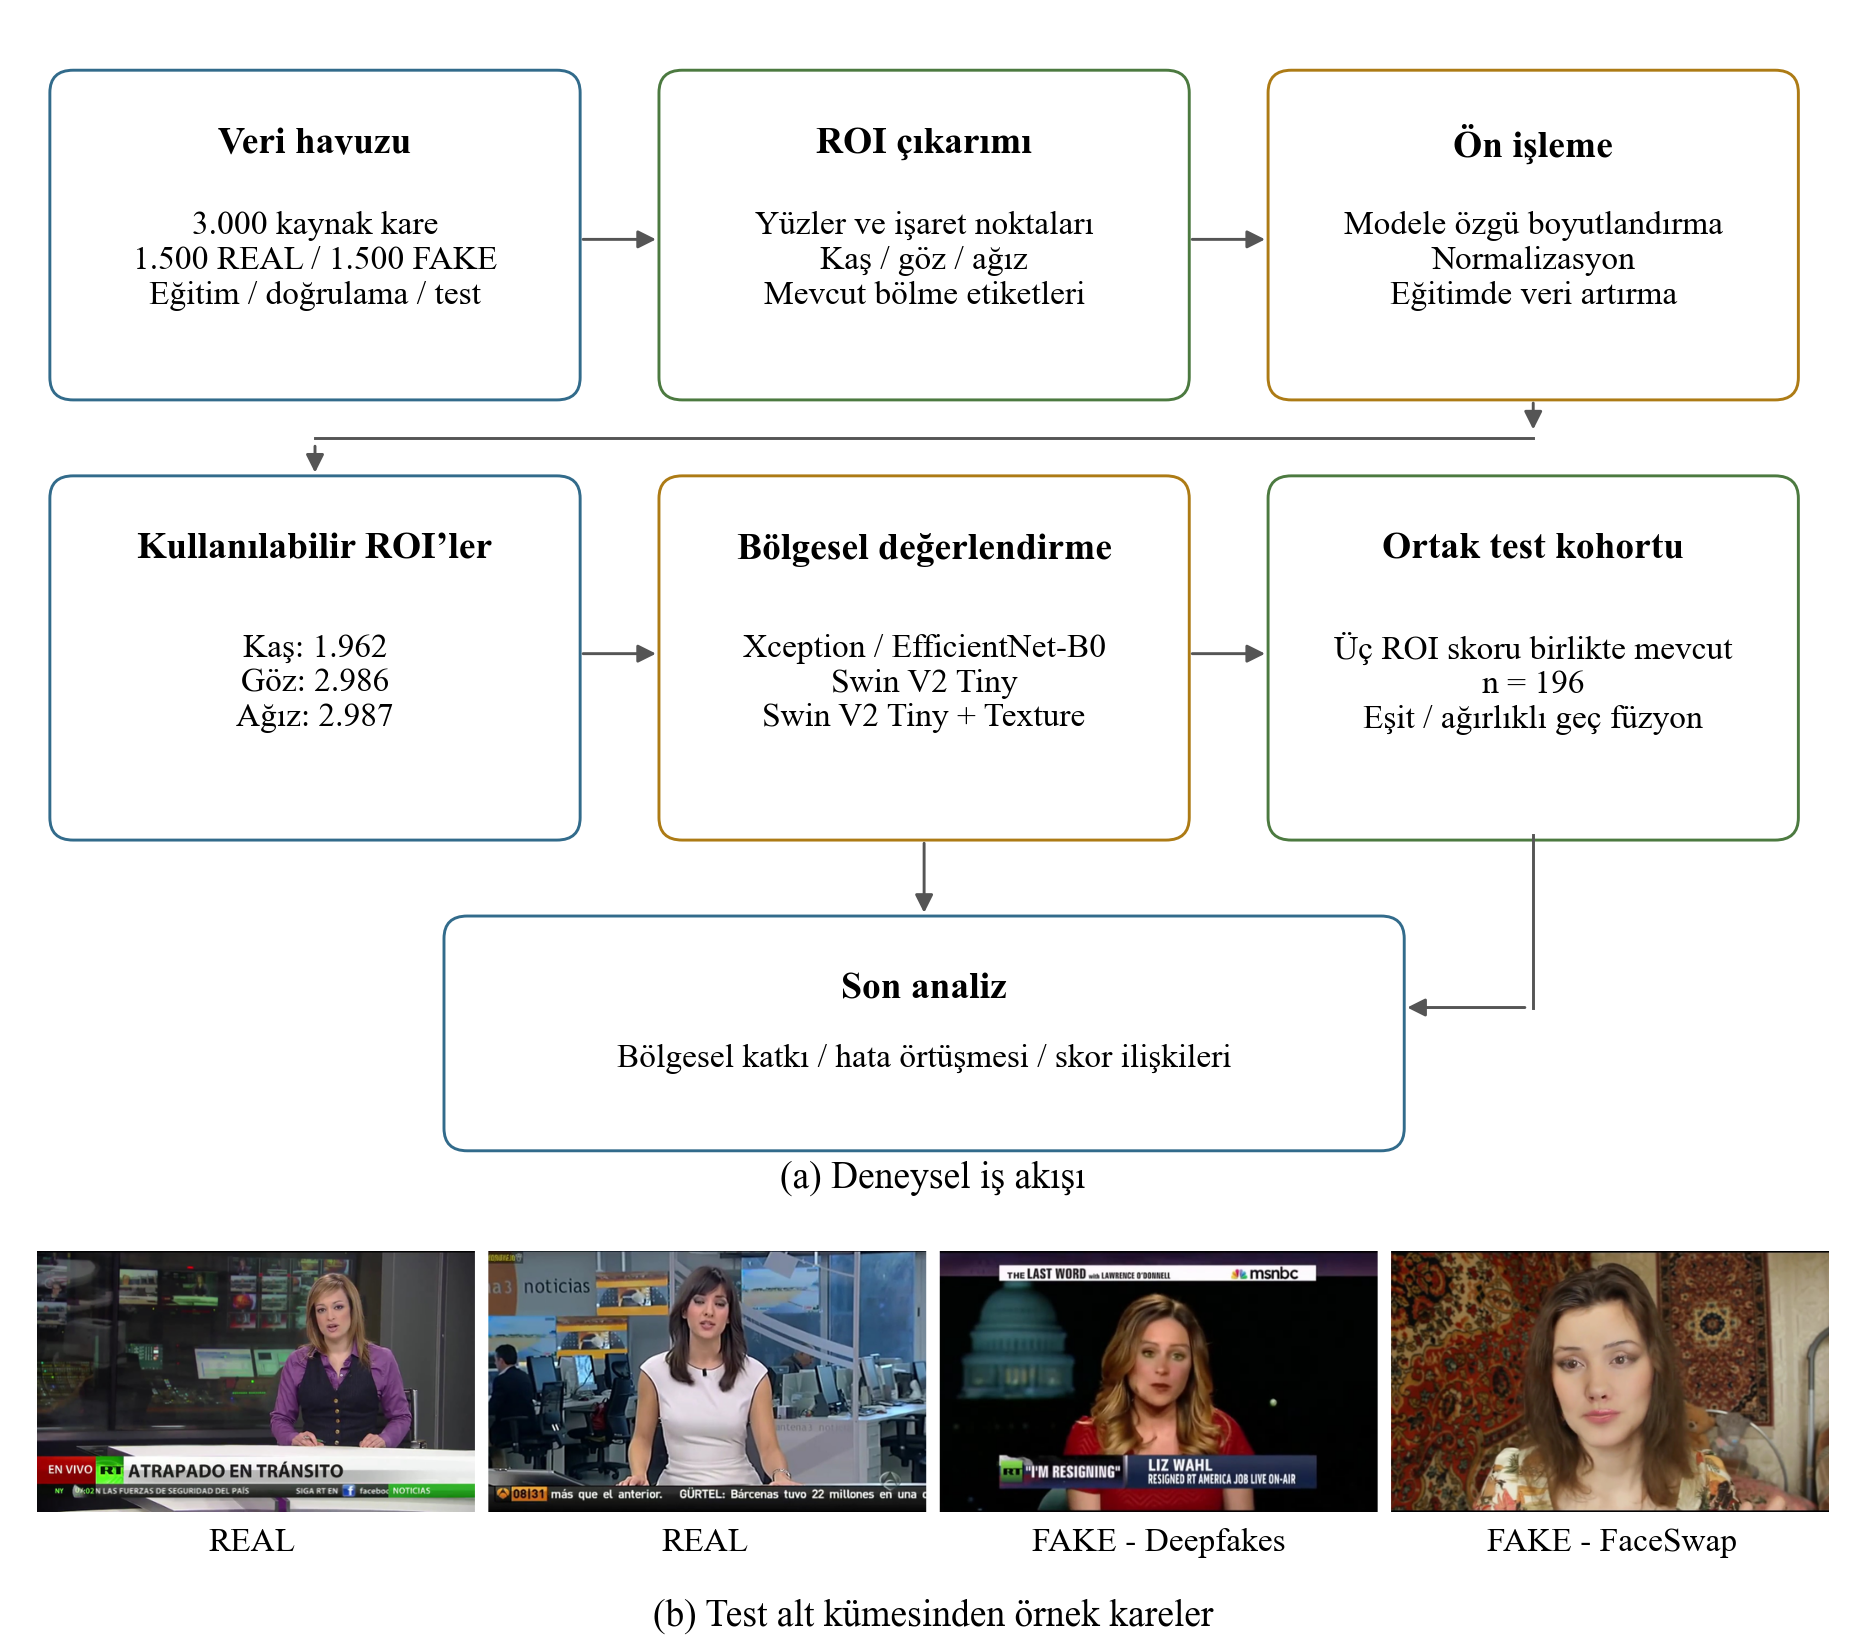
\includegraphics[width=\linewidth]{assets/figure1_complete.png}
\caption{Deney düzeni ve veri örnekleri. (a) Bölgesel değerlendirme ve üç-ROI geç füzyon akışı, (b) soldan sağa iki REAL, bir Deepfakes ve bir FaceSwap örneği.}\label{fig:workflow}
\end{minipage}\end{figure}
Şekil~\ref{fig:workflow}(b)'deki kareler yalnız veri çeşitliliğini örneklemektedir; model için kolay veya zor örnek olarak seçilmemiştir. Şemadaki kaynak düzeyinde bölme, aşağıda açıklanan üst veri kontrolü kapsamında değerlendirilmelidir. Kaynak havuzunun altı manipülasyon etiketi içermesi nedeniyle veri tanımı yalnız standart dört-yöntemli FaceForensics++ alt kümesiyle eş anlamlı değildir.

\subsection{Veri havuzu ve bölme}
FaceForensics proje dağıtımından derlenen havuz 1.500 REAL ve 1.500 FAKE kaynak kare içermektedir. Kaynak kareler yüzde 80/10/10 oranında eğitim, doğrulama ve test bölümlerine ayrılmıştır. Veri bileşimi ve ROI dağılımı Tablo~\ref{tab:data}'da verilmiştir.
\begin{table}[!htbp]\centering\begin{minipage}{15.8cm}
\caption{Kaynak karelerin ve kullanılabilir ROI kayıtlarının dağılımı.}\label{tab:data}
\centering \small
\begin{tabular}{lrrrr}\toprule
Kaynak / bölge & Eğitim & Doğrulama & Test & Toplam \\\midrule
REAL & 1200 & 150 & 150 & 1500 \\
Deepfakes & 190 & 32 & 31 & 253 \\
Face2Face & 208 & 19 & 24 & 251 \\
FaceSwap & 180 & 22 & 20 & 222 \\
NeuralTextures & 163 & 14 & 20 & 197 \\
FaceShifter & 211 & 35 & 31 & 277 \\
DeepFakeDetection & 248 & 28 & 24 & 300 \\
FAKE toplam & 1200 & 150 & 150 & 1500 \\
Kaynak kare toplam & 2400 & 300 & 300 & 3000 \\
\midrule Kaş ROI & 1562 & 204 & 196 & 1962 \\
Göz ROI & 2388 & 296 & 302 & 2986 \\
Ağız ROI & 2389 & 296 & 302 & 2987 \\
\bottomrule\end{tabular}
\par\smallskip\begin{minipage}{\linewidth}\small Kaynak kare sayısı ile ROI kayıt sayısı farklı birimlerdir. Ortak füzyon test kohortu 101 REAL ve 95 FAKE olmak üzere 196 kaynak-kare anahtarından oluşmaktadır.\end{minipage}
\end{minipage}\end{table}

Tablo~\ref{tab:data}'daki FAKE sınıfı altı manipülasyon kaynağından oluşmaktadır. ROI kabul koşulları ve çoklu yüzler nedeniyle ROI sayıları kaynak kare sayılarıyla aynı değildir. Kaşta 1.962, gözde 2.986 ve ağızda 2.987 kullanılabilir kayıt kalmıştır. Kaynak seçim üst verilerinde, aynı sınıftaki özgün kaynak klasörlerinin birden fazla veri bölümünde bulunmadığı belirlenmiştir. Bu kontrol kimlik düzeyinde ayrımı veya aynı gerçek kaynak videodan türetilen bütün farklı manipülasyonların ortak bir kök video kimliğiyle ayrıldığını tek başına kanıtlamaz. ROI kayıtları mevcut veri bölümü etiketlerini korumuştur. Doğrulama verisi model ve kontrol noktası seçimi ile füzyon ağırlıklarının belirlenmesinde, test verisi ise yalnız nihai değerlendirmede kullanılmıştır.

\subsection{ROI çıkarımı ve ön işleme}
Yüz ve işaret noktaları MediaPipe Face Landmarker ile belirlenmiştir. Ağız ROI'si 40 dudak işaret noktası ve çevresel marjla, birleşik göz ROI'si sol ve sağ gözlerin birlikte ele alınmasıyla oluşturulmuştur. Kaş ROI'sinde 20 işaret noktası kullanılmış; en az 48 piksel genişlik, 14 piksel yükseklik ve kırpım içindeki göz işaret noktalarının en fazla 0,25 oranında kalması koşulları uygulanmıştır. Minimum boyut eşikleri çok küçük kaş kırpımlarını elemek, göz noktalarının kapsanma oranına ilişkin eşik ise ROI’nin göz bölgesini aşırı içermesini sınırlandırmak amacıyla uygulanmıştır. Bunlar literatür standardı değil, deney hattının kabul eşikleridir. Görüntüler model gereksinimlerine göre boyutlandırılıp normalize edilmiş; yapılandırmaların çoğunda $224 \times 224$ giriş kullanılmıştır. Veri artırma yalnız eğitim bölümüne uygulanmıştır.

Göz ve ağız test hatlarının her birinde 300 kaynak kareden 310 yüz kaydı oluşmuş; sekiz kayıtta yüz bulunamamış ve 302 başarılı ROI kalmıştır. Kaş hattında 196 başarılı kayıt elde edilmiş, 104 kayıt elenmiştir: 82 yetersiz kaş altı kırpım alanı, 12 yüz bulunamaması, 7 çoklu yüz ve 3 diğer geometrik kontrol. Kaş hattının daha sıkı kabul koşulları hem eğitim verisini hem ortak füzyon kohortunu sınırlamaktadır.

Göz ve ağız test üst verilerinde 10 kare için ikişer başarılı ROI bulunmaktadır. Dokuz karede face00 ve face01 kutuları farklı yüz konumlarına karşılık gelmektedir; \texttt{fake\_test\_00075} için iki kayıt aynı öndeki yüzde büyük ölçüde çakışmaktadır. Bu kare füzyon kohortuna girmemiştir; tam bölgesel test sonuçları bu yinelemeler çıkarılarak yeniden hesaplanmamıştır. Çoklu ROI içeren karelerden yalnız \texttt{fake\_test\_00088} başarılı kaş ROI'siyle ortak kohorta alınmıştır. Bu karede göz ve ağız için face00 skorları kullanılmıştır. Üç face00 kırpımı ana sunucunun aynı yüzüne karşılık gelmektedir. Ortak kohort bu tek-yüz seçim kuralıyla oluşturulmuştur.

\subsection{Model yapılandırmaları ve eğitim}
Xception ve EfficientNet-B0 CNN, Swin V2 Tiny ise Transformer yapılandırmasıdır. Swin V2 Tiny + Texture, görüntü temsillerini LBP, GLCM, Gabor ve dalgacık doku özellikleriyle birleştiren hibrit yapılandırmadır. Modeller ImageNet ön eğitimli ağırlıklarla, ağırlıklı olarak Python ve Google Colab ortamında eğitilmiştir. Tablo~\ref{tab:settings}(a) eğitim ayarlarını; (b) ve (c) panelleri ise sırasıyla doğrulama-temelli füzyon parametrelerini ve bölgesel karar eşiklerini vermektedir.

Hibrit yapılandırmada, Swin V2 Tiny’ın sınıflandırma başlığı kaldırılarak görüntü temsilleri elde edilmiştir. LBP, GLCM, Gabor ve dalgacık tabanlı doku özellikleri, yalnızca eğitim kümesinden öğrenilen standartlaştırma parametreleri kullanılarak ayrı bir doku kolunda işlenmiştir. Görüntü ve doku kollarının çıktıları 256 boyutlu temsillere dönüştürülmüş, ardından özellik düzeyinde birleştirilerek 512 boyutlu tek bir temsil oluşturulmuştur. Bu birleşik temsil ikili sınıflandırıcıya aktarılmıştır.
\begin{table}[!htbp]\centering\begin{minipage}{15.8cm}
\caption{Model eğitim ayarları, füzyon parametreleri ve bölgesel karar eşikleri.}\label{tab:settings}
\centering\small
\textbf{(a) Eğitim ayarları}\par\smallskip
\begin{tabular*}{\linewidth}{@{\extracolsep{\fill}}lrrrr@{}}\toprule
Model & Mini-yığın & Temel LR & Omurga / ince ayar LR & Ağırlık çürümesi\\\midrule
Xception & 16 & $1\times10^{-4}$ & $1\times10^{-5}$ & Göz: $1\times10^{-4}$\\
EfficientNet-B0 &32&$1\times10^{-3}$&$2\times10^{-5}$&$1\times10^{-4}$\\
Swin V2 Tiny &32&$1\times10^{-4}$&$1\times10^{-5}$&$1\times10^{-2}$\\
Swin V2 Tiny + Texture &16&$2\times10^{-4}$&$2\times10^{-5}$&$1\times10^{-4}$\\\bottomrule
\end{tabular*}
\par\medskip
\textbf{(b) Doğrulama ROC-AUC değerleri ve füzyon ağırlıkları}\par\smallskip
\begin{tabular*}{\linewidth}{@{\extracolsep{\fill}}lrrrrrr@{}}\toprule
&\multicolumn{3}{c}{Doğrulama ROC-AUC}&\multicolumn{3}{c}{Füzyon ağırlıkları}\\
Model & Kaş & Göz & Ağız & $w_{\mathrm{brow}}$ & $w_{\mathrm{eye}}$ & $w_{\mathrm{mouth}}$\\\midrule
Xception&0.6710&0.7252&0.8228&0.2378&0.3132&0.4490\\
EfficientNet-B0&0.6819&0.7129&0.7969&0.2630&0.3078&0.4292\\
Swin V2 Tiny&0.7191&0.8454&0.8858&0.2306&0.3634&0.4060\\
Swin V2 Tiny + Texture&0.7280&0.7222&0.8604&0.2812&0.2742&0.4446\\\bottomrule
\end{tabular*}
\par\medskip
\textbf{(c) Bölgesel karar eşikleri}\par\smallskip
\begin{tabular*}{\linewidth}{@{\extracolsep{\fill}}lrrr@{}}\toprule
Model & Kaş & Göz & Ağız\\\midrule
Xception & 0.500 & 0.305 & 0.500\\
EfficientNet-B0 & 0.280 & 0.220 & 0.190\\
Swin V2 Tiny & 0.120 & 0.275 & 0.405\\
Swin V2 Tiny + Texture & 0.330 & 0.265 & 0.455\\\bottomrule
\end{tabular*}
\par\smallskip\begin{minipage}{\linewidth}\small
Xception: dondurulmuş omurga ve ince ayar. EfficientNet-B0: 5 epoch dondurulmuş omurga, 15 epoch ince ayar. Swin V2 Tiny: 20 epoch ve doğrulama ROC-AUC izlemesi; temel LR sınıflandırma başlığına aittir. Hibrit: 30 epoch, son aşamalarda omurganın açılması. LR öğrenme oranıdır; bütün modeller ImageNet ön eğitimlidir. Ağırlıklar gösterim için dört ondalığa yuvarlanmıştır. Xception kaş/ağız kodlarında Adam'a weight decay verilmemiştir; bu sütundaki Xception değeri yalnız göz deneyine aittir. Xception kaş/ağız eşikleri sabit 0,50; diğer bölgesel eşikler doğrulama F1 skoruyla seçilmiştir.
\end{minipage}\end{minipage}\end{table}

Model aileleri için eşit bütçeli sistematik hiperparametre araması yapılmamıştır. Veri artırma ve sınıflandırma başlığı ayarları her model yapılandırması için ayrı ayrı belirlenmiştir. Doğrulama verisinin hem kontrol noktası hem füzyon ağırlığı seçiminde kullanılması doğrulama kümesine uyarlama yanlılığı oluşturabilir.

\subsection{Ortak kohort ve geç füzyon}
Füzyonda bölgesel modeller yeniden eğitilmemiştir. Aynı model ailesinin kaş, göz ve ağız FAKE olasılıkları kaynak-kare anahtarlarıyla eşleştirilmiştir. Üç skorun birlikte mevcut olduğu iç birleşim, 101 REAL ve 95 FAKE içeren 196 kayıt üretmiştir. Ortak küme başarılı kaş test karelerinin tamamını içerir; göz ve ağız tek-bölge sonuçları da aynı anahtarlar üzerinde yeniden hesaplanmıştır.

Eşit füzyon Denklem~\eqref{eq:equal}, doğrulama katkıları ve normalize ağırlıklar Denklem~\eqref{eq:weights}, ağırlıklı füzyon Denklem~\eqref{eq:weighted} ile tanımlanmıştır:
\begin{equation}\label{eq:equal}
P_{\mathrm{equal}}=(P_{\mathrm{brow}}+P_{\mathrm{eye}}+P_{\mathrm{mouth}})/3.
\end{equation}
\begin{equation}\label{eq:weights}
r_i=\max(\mathrm{AUC}^{\mathrm{val}}_i-0.5,\epsilon),\qquad
w_i=\frac{r_i}{\sum_jr_j},\qquad i,j\in\{\mathrm{brow,eye,mouth}\}.
\end{equation}
\begin{equation}\label{eq:weighted}
P_{\mathrm{weighted}}=\sum_iw_iP_i,\qquad\sum_iw_i=1.
\end{equation}
$P_i$ ilgili ROI modelinin FAKE olasılığı, $\mathrm{AUC}^{\mathrm{val}}_i$ doğrulama ROC-AUC değeri ve $\epsilon$ sayısal kararlılık için küçük pozitif sabittir. Ağırlıklar yalnız doğrulama verisinden belirlenmiştir; test bilgisi kullanılmamıştır. Dört modelde de ağız en yüksek ağırlığı almıştır. Ortak kohorttaki hata ve füzyon analizlerinde $P\geq0{,}50$ FAKE kararı olarak kullanılmıştır; tam bölgesel doğruluk/F1 sonuçlarında Tablo~\ref{tab:settings}’deki eşikler geçerlidir.

\subsection{Metrikler, bootstrap ve hata analizi}
Bölgesel karar eşikleri test verisinden seçilmemiştir. Xception kaş/ağız deneylerinde 0,50 sabittir; Xception göz, EfficientNet-B0, Swin V2 Tiny ve hibrit deneylerinde doğrulama F1’ini en yüksek yapan eşik kullanılmıştır. Xception göz, EfficientNet-B0 ve Swin için 0,05--0,95; hibrit için 0,10--0,90 aralığı 0,005 adımlarla taranmıştır. EfficientNet-B0’da eşit F1 durumunda önce yüksek dengeli doğruluk, ardından 0,50’ye yakınlık seçilmiştir; diğer taramalarda ilk maksimum alınmıştır. Seçilen eşik ilgili nihai testte sabitlenmiştir. Ortak kohort hata/füzyon karşılaştırmaları bütün bölgeler için 0,50 kullanır. Ana bölgesel karşılaştırma eşikten bağımsız ROC-AUC’ye dayanmaktadır.

FAKE pozitif, REAL negatif sınıftır. TP/TN doğru pozitif/negatif; FP/FN yanlış pozitif/negatif sayılarıdır. Doğruluk, kesinlik, duyarlılık, özgüllük, F1 ve dengeli doğruluk Denklem~\eqref{eq:metrics} ile hesaplanmıştır:
\begin{equation}\label{eq:metrics}
\begin{aligned}
\mathrm{Doğruluk}&=\frac{TP+TN}{TP+TN+FP+FN},&
\mathrm{Kesinlik}&=\frac{TP}{TP+FP},\\
\mathrm{Duyarlılık}&=\frac{TP}{TP+FN},&
\mathrm{Özgüllük}&=\frac{TN}{TN+FP},\\
\mathrm{F1}&=\frac{2TP}{2TP+FP+FN},&
\mathrm{Dengeli\ doğruluk}&=\frac{\mathrm{Duyarlılık}+\mathrm{Özgüllük}}{2}.
\end{aligned}
\end{equation}
Alıcı işletim karakteristiği eğrisinin altında kalan alan (ROC-AUC) eşikten bağımsız temel karşılaştırma ölçütüdür; kesinlik--duyarlılık eğrisinin altında kalan alan (PR-AUC) kesinlik--duyarlılık performansını özetler. Eşik bağımlı karar sayılarıyla ROC-AUC sıralama performansı ayrı kavramlardır.

Füzyon farkı $\Delta\mathrm{AUC}=\mathrm{AUC}_{\mathrm{füzyon}}-\mathrm{AUC}_{\mathrm{ağız}}$ olarak tanımlanmıştır. Ortak kohortta rastgelelik tohumu 42 ile 5.000 tekrarlı örnek düzeyinde eşleştirilmiş bootstrap uygulanmış; her tekrarda aynı indeksler ağız ve füzyon skorlarına verilmiştir. Tek sınıflı yeniden örneklemeler dışlanmış, yüzde 95 güven aralıkları dağılımın 2,5 ve 97,5 yüzdeliklerinden elde edilmiştir. Sekiz karşılaştırmaya çoklu karşılaştırma düzeltmesi uygulanmamıştır. Örnek düzeyindeki yeniden örnekleme, aynı videonun kareleri arasındaki bağımlılığı modellememektedir.

Hata analizinde her ROI için 0,50 eşikte doğru/yanlış vektörü oluşturulmuş ve üç ROI'nin sekiz birbirini dışlayan kombinasyonu sayılmıştır. Ağız yanlışken füzyonun doğruya çevirdiği örnekler ``kurtarılan'', ağız doğruyken füzyonun yanlış karara çevirdiği örnekler ``bozulan'' olarak tanımlanmıştır. Net etki kurtarılan eksi bozulan örnek sayısıdır. Skor ilişkileri Spearman sıra korelasyonu ile incelenmiştir; düşük korelasyon tek başına yararlı tamamlayıcılığı kanıtlamaz.

\section{Bulgular}
\subsection{Bölgesel sonuçlar}
Tablo~\ref{tab:regional}, tam bölgesel test kümelerindeki doğruluk, F1 ve ROC-AUC ile ortak kohortta yeniden hesaplanan ROC-AUC değerlerini birlikte sunmaktadır. Kaşın tam testi ve ortak kohort 196; göz ve ağzın tam testleri 302 örnek içerir. Tam test ile ortak kohort arasındaki değer farkları farklı örnek kümelerinden kaynaklanmaktadır.
\begin{table}[!htbp]\centering\begin{minipage}{15.8cm}
\caption{Tam bölgesel testler ve ortak kohorttaki bölgesel performans.}\label{tab:regional}
\centering \small
\begin{tabular}{llrrrr}\toprule
Model & ROI & Doğruluk (\%) & F1 (\%) & Tam-test AUC & Ortak AUC \\\midrule
Xception & Kaş & 51.53 & 55.81 & 0.5513 & 0.5513 \\
 & Göz & 57.28 & 70.34 & 0.6770 & 0.6668 \\
 & Ağız & 70.20 & 72.22 & 0.7662 & 0.7527 \\
EfficientNet-B0 & Kaş & 54.59 & 65.10 & 0.5874 & 0.5874 \\
 & Göz & 63.58 & 72.08 & 0.7286 & 0.7313 \\
 & Ağız & 71.52 & 76.76 & 0.8332 & 0.8334 \\
Swin V2 Tiny & Kaş & 53.57 & 65.92 & 0.6815 & 0.6815 \\
 & Göz & 69.87 & 72.84 & 0.7868 & 0.7829 \\
 & Ağız & 80.46 & 80.91 & 0.8607 & 0.8803 \\
Swin V2 Tiny + Texture & Kaş & 60.20 & 67.23 & 0.6688 & 0.6688 \\
 & Göz & 61.26 & 69.77 & 0.7090 & 0.6756 \\
 & Ağız & 71.85 & 74.47 & 0.7918 & 0.7897 \\
\bottomrule\end{tabular}
\par\smallskip\begin{minipage}{\linewidth}\small Tam-test sayıları: kaş 196, göz ve ağız 302. Ortak kohort: 196 (101 REAL, 95 FAKE). Doğruluk/F1, Tablo~\ref{tab:settings}’deki bölgesel eşiklerle hesaplanmıştır; ortak kohort hata/füzyon analizleri 0,50 kullanır. Eşik bağımlı metrikler yüzde; ROC-AUC değerleri 0--1 ölçeğindedir.\end{minipage}
\end{minipage}\end{table}

Dört yapılandırmanın tamamında hem tam test hem ortak kohort AUC nokta tahminleri ağız $>$ göz $>$ kaş biçimindedir. Swin V2 Tiny tam testte kaş, göz ve ağız için sırasıyla 0,6815, 0,7868 ve 0,8607 ile en yüksek AUC değerlerini üretmiştir. EfficientNet-B0'ın ağız AUC'si 0,8332'dir. Hibrit model kaşta yüzde 60,20 doğruluk ve yüzde 67,23 F1 ile en yüksek eşik bağımlı sonuçları vermiş; ancak üç ROI'nin tamamında AUC'si temel Swin'in altında kalmıştır. Farklı eşik seçim kurallarında elde edilen doğruluk/F1 sonuçları saf mimari üstünlük kanıtı değildir; temel karşılaştırma ROC-AUC üzerinden yapılmıştır.

Swin V2 Tiny'ın ağız, göz ve kaş için tam-test ROC eğrileri sırasıyla Şekil~\ref{fig:roc}(a), \ref{fig:roc}(b) ve \ref{fig:roc}(c)'de verilmiştir. Ağız modeli en yüksek AUC değerine sahiptir; AUC sıralaması ROC eğrilerinin her eşikte birbirine üstün olduğu anlamına gelmez.
\begin{figure}[!htbp]\centering\begin{minipage}{15.8cm}\centering
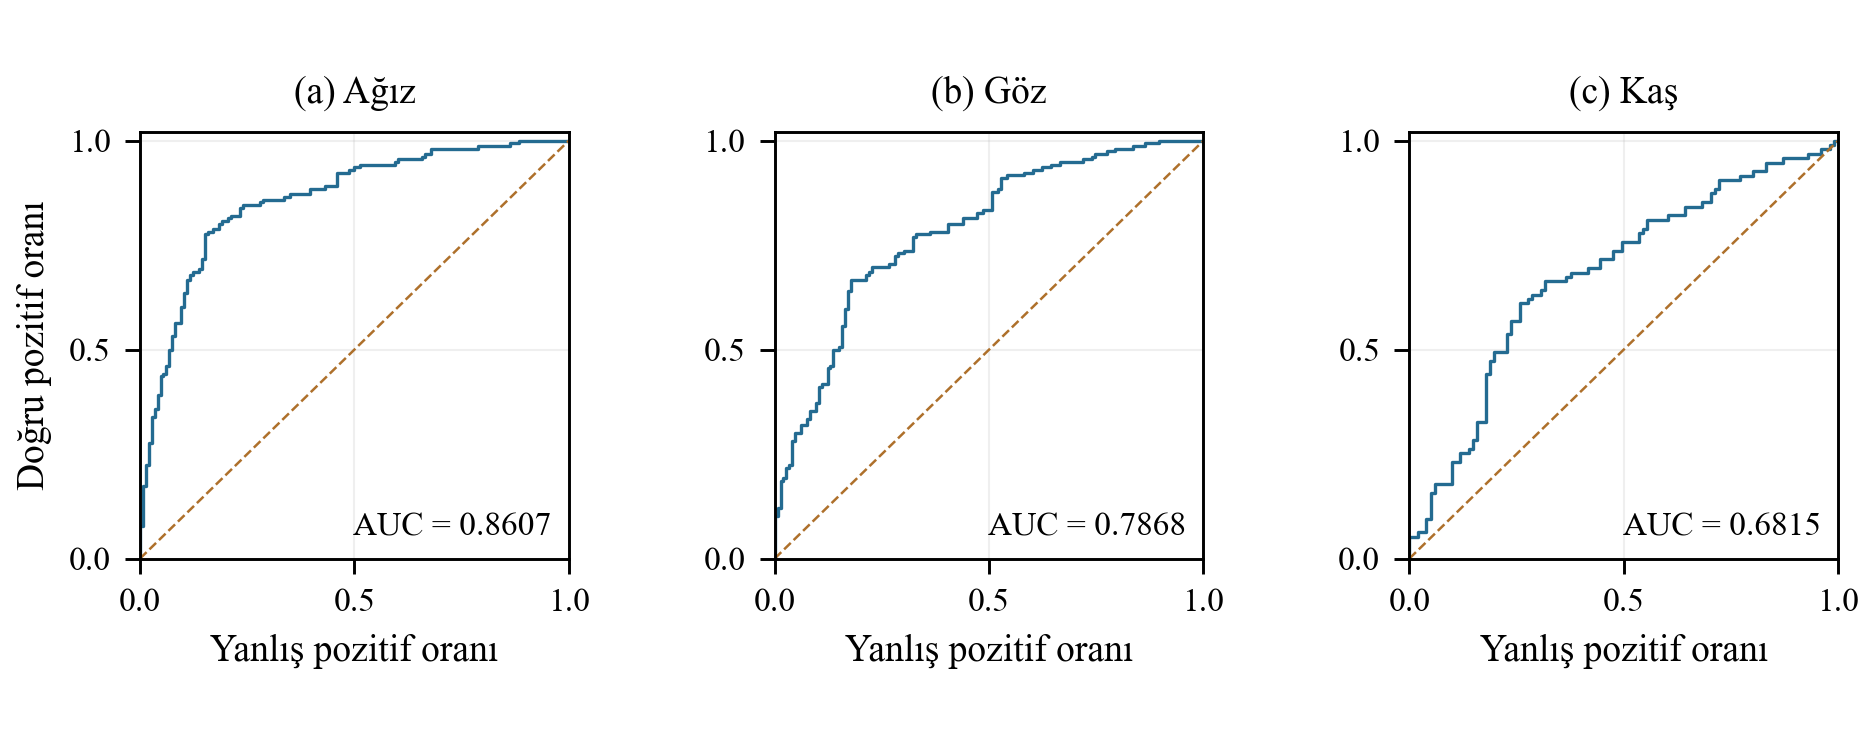
\includegraphics[width=\linewidth]{assets/roc_combined.png}
\caption{Swin V2 Tiny için tam-test ROC eğrileri. (a) Ağız, (b) göz, (c) kaş.}\label{fig:roc}
\end{minipage}\end{figure}

Veri bileşimiyle bölgesel performansın ilişkisi, Swin V2 Tiny için mevcut keşifsel manipülasyon alt grubu sonuçlarıyla incelenmiştir (Tablo~\ref{tab:subgroup}). Her FAKE alt grubu aynı 101 REAL örnekle karşılaştırılmıştır.
\begin{table}[!htbp]\centering\begin{minipage}{15.8cm}
\caption{Swin V2 Tiny için ortak kohortta keşifsel manipülasyon alt grubu ROC-AUC değerleri.}\label{tab:subgroup}
\centering \small
\begin{tabular}{lrrrr}\toprule
Manipülasyon & FAKE sayısı & Kaş AUC & Göz AUC & Ağız AUC \\\midrule
Deepfakes & 21 & 0.6841 & 0.9128 & 0.8689 \\
FaceShifter & 24 & 0.8156 & 0.8412 & 0.9068 \\
NeuralTextures & 13 & 0.5598 & 0.5385 & 0.8576 \\
Face2Face & 17 & 0.6500 & 0.7443 & 0.8567 \\
FaceSwap & 14 & 0.4767 & 0.6690 & 0.8501 \\
DeepFakeDetection & 6 & 0.9670 & 1.0000 & 1.0000 \\
\bottomrule\end{tabular}
\par\smallskip\begin{minipage}{\linewidth}\small Her satırda 101 REAL örnek kullanılmıştır. Küçük FAKE alt grupları nedeniyle değerler doğrulayıcı bir manipülasyonlar-arası üstünlük testi değildir.\end{minipage}
\end{minipage}\end{table}

Ağız dört alt grupta en yüksek AUC'yi vermiş; Deepfakes'te göz daha yüksek çıkmıştır. DeepFakeDetection'daki göz ve ağız AUC'si 1,0000 olmakla birlikte yalnız altı FAKE örnek vardır. Bu değer tüm manipülasyonlar için kusursuz tespit iddiasına dönüştürülemez.

\subsection{Geç füzyon ve belirsizlik}
Tablo~\ref{tab:fusion}(a) ve (b), sırasıyla eşik bağımlı ve eşikten bağımsız füzyon metriklerini; (c) paneli ise yalnız ağız sonucuna göre eşleştirilmiş AUC farklarını ve bunların güven aralıklarını vermektedir. Böylece ROC-AUC, PR-AUC ve eşik bağımlı sonuçlar farklı test kümeleriyle karıştırılmadan izlenebilir.
\begin{table}[!htbp]\centering\begin{minipage}{15.8cm}
\caption{Ortak kohorttaki füzyon performansı ve yalnız ağız karşılaştırması.}\label{tab:fusion}
\centering\small
\textbf{(a) Eşik bağımlı füzyon metrikleri (\%)}\par\smallskip
\begin{tabular*}{\linewidth}{@{\extracolsep{\fill}}llrrrrrr@{}}\toprule
Model & Füzyon & Doğr. & Deng. & Kes. & Duy. & Özg. & F1 \\\midrule
Xception & Eşit & 63.78 & 64.04 & 60.53 & 72.63 & 55.45 & 66.03 \\
 & Ağırlıklı & 68.88 & 69.05 & 65.74 & 74.74 & 63.37 & 69.95 \\
EfficientNet-B0 & Eşit & 72.45 & 72.39 & 72.04 & 70.53 & 74.26 & 71.28 \\
 & Ağırlıklı & 73.47 & 73.44 & 72.63 & 72.63 & 74.26 & 72.63 \\
Swin V2 Tiny & Eşit & 77.04 & 76.82 & 80.49 & 69.47 & 84.16 & 74.58 \\
 & Ağırlıklı & 79.59 & 79.39 & 83.13 & 72.63 & 86.14 & 77.53 \\
Swin V2 Tiny + Texture & Eşit & 69.39 & 69.20 & 70.59 & 63.16 & 75.25 & 66.67 \\
 & Ağırlıklı & 68.88 & 68.74 & 69.32 & 64.21 & 73.27 & 66.67 \\
\bottomrule\end{tabular*}
\par\medskip
\textbf{(b) Eşikten bağımsız füzyon metrikleri}\par\smallskip
\begin{tabular*}{\linewidth}{@{\extracolsep{\fill}}llrr@{}}\toprule
Model & Füzyon & ROC-AUC & PR-AUC \\\midrule
Xception & Eşit & 0.7164 & 0.6808 \\
 & Ağırlıklı & 0.7412 & 0.6922 \\
EfficientNet-B0 & Eşit & 0.8017 & 0.8055 \\
 & Ağırlıklı & 0.8196 & 0.8232 \\
Swin V2 Tiny & Eşit & 0.8587 & 0.8652 \\
 & Ağırlıklı & 0.8763 & 0.8803 \\
Swin V2 Tiny + Texture & Eşit & 0.7523 & 0.7361 \\
 & Ağırlıklı & 0.7672 & 0.7484 \\
\bottomrule\end{tabular*}
\par\medskip
\textbf{(c) Yalnız ağız sonucuna göre eşleştirilmiş ROC-AUC farkları}\par\smallskip
\begin{tabular*}{\linewidth}{@{\extracolsep{\fill}}llrrrr@{}}
\toprule
Model & Füzyon & Ağız AUC & Füzyon AUC & $\Delta$AUC & \%95 GA ($\Delta$AUC)\\\midrule
Xception & Eşit & 0.7527 & 0.7164 & -0.0363 & [-0.0839; 0.0101] \\
 & Ağırlıklı & 0.7527 & 0.7412 & -0.0115 & [-0.0455; 0.0226] \\
EfficientNet-B0 & Eşit & 0.8334 & 0.8017 & -0.0317 & [-0.0752; 0.0102] \\
 & Ağırlıklı & 0.8334 & 0.8196 & -0.0138 & [-0.0471; 0.0204] \\
Swin V2 Tiny & Eşit & 0.8803 & 0.8587 & -0.0216 & [-0.0675; 0.0237] \\
 & Ağırlıklı & 0.8803 & 0.8763 & -0.0040 & [-0.0434; 0.0367] \\
Swin V2 Tiny + Texture & Eşit & 0.7897 & 0.7523 & -0.0374 & [-0.0933; 0.0174] \\
 & Ağırlıklı & 0.7897 & 0.7672 & -0.0225 & [-0.0700; 0.0236] \\\bottomrule
\end{tabular*}
\par\smallskip\small
Doğr.: doğruluk; Deng.: dengeli doğruluk; Kes.: kesinlik; Duy.: duyarlılık; Özg.: özgüllük. Panel (a) yüzde, paneller (b) ve (c) AUC değerlerini verir. Tüm satırlarda $n = 196$; eşik bağımlı sonuçlarda eşik 0,50 kullanılmıştır. GA güven aralığıdır.
\end{minipage}\end{table}

Ağırlıklı füzyon dört modelde de eşit füzyondan daha yüksek ROC-AUC nokta tahmini vermiştir. En yüksek füzyon değeri Swin V2 Tiny için 0,8763'tür. Ancak hem eşit hem ağırlıklı füzyon, her modelin ortak kohorttaki ağız AUC'sinin altında kalmıştır. Hibrit modelde ağırlıklı füzyonun AUC'si artarken doğruluk yüzde 69,39'dan yüzde 68,88'e düşmüştür; dolayısıyla iyileşme ifadesi bütün metriklere genellenemez.

Sekiz $\Delta$AUC güven aralığı da sıfırı içermektedir. Swin V2 Tiny ağırlıklı füzyonunda fark -0,0040 ve yüzde 95 güven aralığı [-0,0434; 0,0367]'dir. Mevcut örneklemde ek füzyon kazancı gösterilememiştir; bu bulgu yaklaşımların eşdeğer olduğunu veya küçük pozitif bir farkın olanaksız olduğunu kanıtlamaz. Füzyonun ağızdan istatistiksel olarak daha kötü olduğu iddiası da bu aralıklardan çıkarılamaz.

\subsection{Hata örüntüleri ve skor ilişkileri}
Tablo~\ref{tab:errors}(a) üç ROI'nin sekiz doğru/yanlış kombinasyonunu, (b) paneli ise ağız--füzyon karar değişimlerini göstermektedir. İkili kategorilerde adı geçmeyen üçüncü ROI yanlıştır; sekiz kategori birbirini dışlar ve satır toplamları 196'dır.
\begin{table}[!htbp]\centering\begin{minipage}{15.8cm}
\caption{Ortak kohortta ROI karar kombinasyonları ve füzyonun kazanç/kayıp sayıları.}\label{tab:errors}
\centering \small
\textbf{(a) ROI karar kombinasyonları}\par\smallskip
\begin{tabular*}{\linewidth}{@{\extracolsep{\fill}}lrrrrrrrr@{}}\toprule
Model & Yalnız A & Yalnız G & Yalnız K & A+G & A+K & G+K & \shortstack{Üçü\\doğru} & \shortstack{Üçü\\yanlış} \\\midrule
Xception & 22 & 11 & 8 & 35 & 15 & 12 & 66 & 27 \\
EfficientNet-B0 & 24 & 9 & 6 & 35 & 14 & 13 & 75 & 20 \\
Swin V2 Tiny & 16 & 8 & 4 & 30 & 19 & 15 & 93 & 11 \\
Swin V2 Tiny + Texture & 23 & 10 & 10 & 22 & 18 & 15 & 79 & 19 \\
\bottomrule\end{tabular*}
\par\smallskip\begin{minipage}{\linewidth}\small A: ağız, G: göz, K: kaş. Her iki panelde karar eşiği 0,50’dir. Bölgesel doğruluk/F1 sonuçları Tablo~\ref{tab:settings}’deki eşikleri kullandığından kaş doğru toplamları farklı olabilir.\end{minipage}
\par\medskip\small\textbf{(b) Ağızdan füzyona karar değişimleri}\par\smallskip
\begin{tabular*}{\linewidth}{@{\extracolsep{\fill}}lrrrrrrrr@{}}\toprule
 & \multicolumn{2}{c}{Ağız} & \multicolumn{3}{c}{Eşit füzyon} & \multicolumn{3}{c}{Ağırlıklı füzyon}\\
Model & Doğru & Yanlış & Kurtardı & Bozdu & Net & Kurtardı & Bozdu & Net\\\midrule
Xception & 138 & 58 & 11 & 24 & -13 & 9 & 12 & -3 \\
EfficientNet-B0 & 148 & 48 & 12 & 18 & -6 & 11 & 15 & -4 \\
Swin V2 Tiny & 158 & 38 & 14 & 21 & -7 & 13 & 15 & -2 \\
Swin V2 Tiny + Texture & 142 & 54 & 16 & 22 & -6 & 12 & 19 & -7 \\\bottomrule\end{tabular*}\end{minipage}\end{table}

Karar değişimi tablosunda Swin V2 Tiny ağız modeli 158 doğru ve 38 yanlış karar vermiştir. Ağırlıklı füzyon 13 ağız hatasını düzeltirken 15 doğru kararı bozmuş; net değişim $13-15=-2$ olmuştur. Bu sayı 0,50 eşikte doğru sınıflandırılan örnekleri açıklamakta, AUC farkının doğrudan hesabı yerine geçmemektedir. Diğer modellerde de raporlanan ağırlıklı füzyon net etkileri negatiftir.

Kaş için Swin V2 Tiny’ın 0,12 bölgesel eşikte 105, ortak analizdeki 0,50 eşikte 131 doğru kararı vardır. EfficientNet-B0’da 0,28/0,50 eşiklerinde 107/108, hibritte 0,33/0,50 eşiklerinde 118/122 doğru karar elde edilmektedir. Her iki değerlendirmede de aynı 196 örnek, aynı etiketler ve aynı kaş olasılıkları kullanılmıştır; sonuçlar arasındaki fark karar eşiğinden kaynaklanmaktadır.

Ortak kohorttaki skor ilişkileri Xception, EfficientNet-B0, Swin V2 Tiny ve hibrit model için sırasıyla Şekil~\ref{fig:corr}(a), \ref{fig:corr}(b), \ref{fig:corr}(c) ve \ref{fig:corr}(d)'de gösterilmiştir. Ağız--göz Spearman katsayıları Xception, EfficientNet-B0, Swin V2 Tiny ve hibrit model için sırasıyla 0,428, 0,482, 0,518 ve 0,440; ağız--kaş katsayıları 0,253, 0,320, 0,381 ve 0,482'dir. Göz--kaş katsayıları sırasıyla 0,477, 0,459, 0,585 ve 0,585'tir. Bölgeler aynı örnekleri birebir aynı biçimde sıralamamaktadır. Bu gözlem farklı skor davranışlarını gösterir; nedensel açıklama veya otomatik füzyon kazancı kanıtı değildir.
\begin{figure}[!htbp]\centering\begin{minipage}{15.8cm}\centering
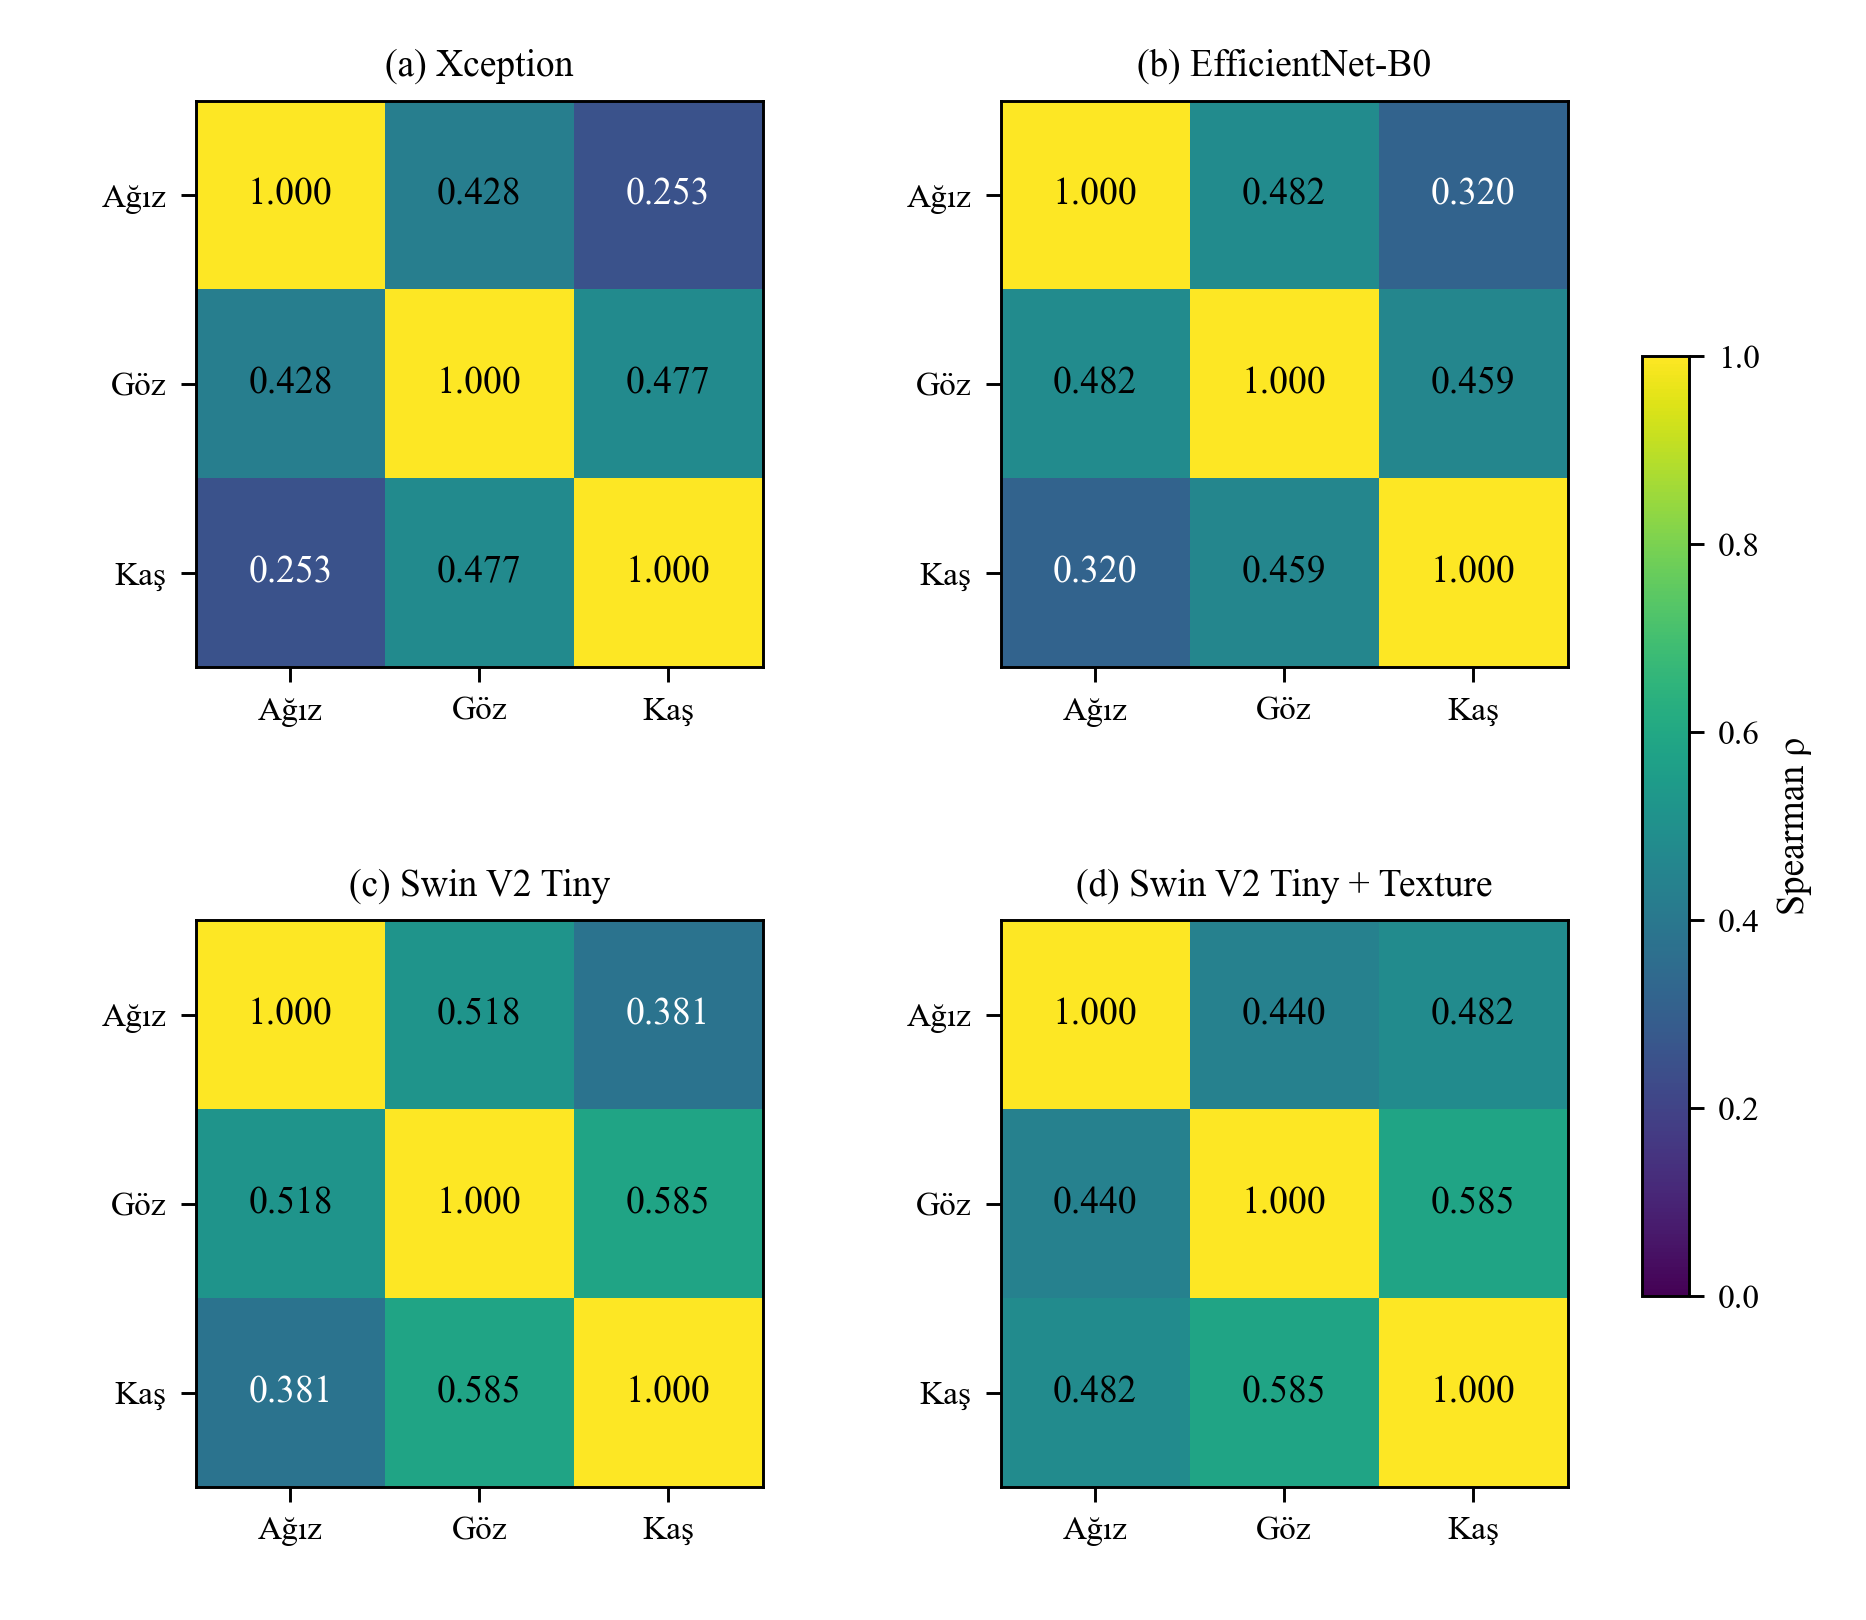
\includegraphics[width=\linewidth]{assets/correlations.png}
\caption{Ortak kohortta bölgesel FAKE olasılıklarının Spearman korelasyonları. (a) Xception, (b) EfficientNet-B0, (c) Swin V2 Tiny, (d) Swin V2 Tiny + Texture.}\label{fig:corr}
\end{minipage}\end{figure}

\section{Tartışma}
Ağız ROI'sinin dört yapılandırmada daha yüksek AUC üretmesi, bu kaynak havuzunda ağız görünümünün ayırt edici bilgi taşıdığını düşündürmektedir. Dudak sınırları, dişler ve ağız içi dokular olası ipuçlarıdır; ancak mevcut deneylerde bunların katkıları ayrı ayrı ölçülmemiştir. Tolosana ve arkadaşlarının farklı veri kümelerinde değişen bölgesel sonuçları \cite{tolosana}, gözlenen ağız avantajının evrensel bir anatomik üstünlük olarak sunulmaması gerektiğini desteklemektedir. Manipülasyon-alt-grup sonuçları da tek tip davranış göstermemektedir.

Ağız hareketi kullanan LipForensics ve DFT-MF \cite{haliassos,elhassan} ile öğrenilebilir uzamsal-zamansal özellik işlemleri kullanan Mirzayev ve Dibeklioğlu \cite{mirzayev}, statik karelerin dışında bilgi kaynakları incelemektedir. Buradaki ağız sonucu hareket modellemesine bağlanamaz. Göz kırpma analizleri \cite{li,jung} de mevcut statik göz deneylerinin kapsamadığı davranışsal bilgiyi kullanır. Kaşın daha düşük performansı azalan ROI sayısı ve kırpım koşullarıyla ilişkili olabilir; veri miktarı ve ROI kalitesinin nedensel etkileri ayrı ayrı incelenmemiştir.

Swin V2 Tiny'ın üç bölgede de en yüksek AUC'yi vermesine karşılık hibrit doku yapılandırması temel Swin'i aşmamıştır. Bu sonuç bütün doku özelliklerinin zararlı olduğu anlamına gelmez. Eğitim ayarları ve kullanılan uzamsal kapsam farklı olabilir; LBP, GLCM, Gabor ve dalgacık için ayrı bileşen çıkarma analizi bulunmamaktadır. Shivaprakash ve arkadaşlarının yüksek hibrit sonuçları \cite{shivaprakash}, farklı veri ve protokolde raporlandığından mevcut yerel ROI sonuçlarıyla doğrudan üstünlük sıralamasına dönüştürülmemelidir.

Füzyon için ağırlıklandırma kuralı tek bir ROI'ye bağlı olmayan, doğrulama performansıyla belirlenen bir birleşim sağlamıştır. Buna rağmen sabit ağırlıklar, her örnekte hangi ROI'nin güvenilir olduğunu modellememektedir. Bazı ağız hataları düzelirken bazı doğru ağız kararlarının bozulması, tamamlayıcılığın otomatik olarak toplam kazanca dönüşmediğini göstermektedir. Eğitim sonrası olasılık kalibrasyonu yapılmadığından skor ölçekleri ve güven farklılıkları olası bir etkendir; bu açıklama mevcut sonuçlarla doğrulanmış bir neden değil, gelecek çalışmada sınanabilecek bir hipotezdir. Yerel manipülasyonlar için çapraz dikkat temelli temsil füzyonu \cite{anand} ve farklı özellik dallarının birleşimi \cite{lei}, sabit ROI skoru ortalamasından farklı tasarımlar sunduğu için sonuçlar bütün füzyon yöntemlerine genellenemez.

Yakın çalışmalarla karşılaştırma Tablo~\ref{tab:literature}'de özetlenmiştir. Sayılar farklı veri kümeleri, ROI tanımları, zamansal bilgi ve metrikler altında elde edilmiştir; tablo yöntemsel bağlam sunmaktadır.
\begin{table}[!htbp]\centering\begin{minipage}{15.8cm}
\caption{Yakın çalışmaların yöntem ve bulgularıyla karşılaştırma.}\label{tab:literature}
\centering \small
\begin{tabular}{>{\raggedright\arraybackslash}p{2.2cm}>{\raggedright\arraybackslash}p{3.0cm}>{\raggedright\arraybackslash}p{4.1cm}>{\raggedright\arraybackslash}p{4.1cm}}\toprule
Çalışma & Yöntem / kapsam & Raporlanan sonuç & Karşılaştırmanın sınırı \\\midrule
Tolosana ve ark. \cite{tolosana} & Bölgesel Xception / Capsule; UADFV, FF++, Celeb-DF, DFDC Preview. & Xception ağız AUC: 0,954 / 0,939 / 0,651 / 0,795. & Bölgesel güç veri kümesine bağlıdır. Burada Xception tam-test ağız AUC: 0,7662. \\
Haliassos ve ark. \cite{haliassos} & LipForensics; zamansal ağız dinamikleri. & Video düzeyinde doğruluk: FF++ HQ/LQ yüzde 98,8 / 94,2; çapraz-veri AUC: Celeb-DF v2 0,824; DFDC 0,735. & Mevcut statik ağız ROI’sinden farklı bilgi ve protokol kullanır. \\
Nguyen ve Derakhshani \cite{nguyen} & Kaş biyometrisi; Celeb-DF ve VISOB. & Yaklaşık 0,88 AUC ve yüzde 20,7 EER. & Kimlik eşleştirmesi ile statik ROI sınıflandırması aynı görev değildir. \\
Soudy ve ark. \cite{soudy} & Göz/burun/tüm yüz; CNN/CViT ve çoğunluk oylaması. & Göz CNN modellerinde yaklaşık yüzde 96 / 97; tüm-yüz CViT deneyinde yüzde 85 doğruluk. & Farklı bölgeler, karar füzyonu ve metrik kullanır; mevcut AUC ile doğrudan sıralanamaz. \\
Lei ve ark. \cite{lei} & Geliştirilmiş MTCNN tabanlı yüz tespiti, difüzyon ön işleme, geometri/doku ve karar füzyonu. & Çok özellikli tespit ve adversarial savunma çerçevesi. & Üç anatomik ROI’nin aynı kohortta skor füzyonu karşılaştırmasından farklıdır. \\
Shivaprakash ve ark. \cite{shivaprakash} & Swin V2 ve LBP, GLCM, Gabor ve dalgacık. & FF++ AUC 0,9929; Celeb-DF v2 AUC 0,9962. & Bu protokolde hibrit ROI modeli temel Swin’i AUC’de aşmamıştır. \\
Mirzayev ve Dibeklioğlu \cite{mirzayev} & Hareket büyütme ağlarından esinlenen öğrenilebilir özellik işlemleri. & Uzamsal-zamansal tutarsızlıkları inceleyen video tespiti. & Zamansal temsil, mevcut statik kare deneyinin dışındadır. \\
Bu çalışma & Üç ROI, dört yapılandırma ve ortak 196 örnekte geç füzyon. & Swin ağız: tam-test 0,8607; ortak 0,8803. Ortak ağırlıklı füzyon: 0,8763. & Eşit/ağırlıklı füzyon için ağız üzerine ek AUC kazancı gösterilememiştir. \\
\bottomrule\end{tabular}
\par\smallskip\begin{minipage}{\linewidth}\small EER: eşit hata oranı; HQ/LQ: yüksek/düşük kalite; FF++: FaceForensics++; DFDC: Deepfake Detection Challenge; CViT: evrişimli görsel Transformer; MTCNN: çok görevli kademeli evrişimli sinir ağı. Dış sonuçlar farklı protokollere aittir; ortak veri üzerinde yeniden değerlendirme veya doğrudan üstünlük karşılaştırması yapılmamıştır.\end{minipage}
\end{minipage}\end{table}

\subsection{Sınırlılıklar}
Çalışma tek bir FaceForensics proje havuzu ve deney protokolüyle sınırlıdır; bağımsız veri kümesinde veri kümeleri arası test yapılmamıştır. Ortak füzyon kohortunun 196 örnekle sınırlı olması, özellikle küçük AUC farklarının belirlenmesini güçleştirmektedir. Kaşın düşük ROI kullanılabilirliği değerlendirmeyi geometrik koşulları sağlayan alt kümeye yöneltmekte ve tüm kaynak kareleri temsil etmeyebilmektedir.

Kaynak klasör/veri bölümü kontrolü kimlik veya tüm manipülasyonlar boyunca ortak kök-video düzeyinde ayrım için tam kanıt değildir. Örnek düzeyindeki bootstrap video bağımlılığını dikkate almaz; güven aralıkları iyimser olabilir. Bölgeler arası AUC farkları için ayrıca güven aralığı hesaplanmadığından ağız--göz--kaş sıralaması nokta tahminleriyle sınırlıdır. Tam göz/ağız testinde çakışan ROI kayıtları bulunması değerlendirmenin bağımlılık yapısını etkileyebilir. Modele özgü eşik seçim kuralları doğruluk/F1 karşılaştırmalarını sınırlar; bu metrikler doğrudan mimari üstünlük kanıtı olarak yorumlanmamalıdır.

Statik kareler göz kırpma veya dudak hareketini modellememektedir. Tüm-yüz karşılaştırma modeli, hibrit bileşen çıkarma analizi, eğitim sonrası kalibrasyon ve standart donanımda ortak maliyet ölçümü bulunmamaktadır. Eğitim bütçeleri eşitlenmediğinden sonuçlar saf mimari üstünlük kanıtı değildir. Alan genellemesine ilişkin yöntemsel çalışmalar \cite{karimi}, haricî veri değerlendirmesinin neden ayrıca gerekli olduğunu desteklemektedir.

\section{Sonuç ve gelecek çalışmalar}
Mevcut protokolde ağız ROI'si dört model yapılandırmasında en yüksek bölgesel ROC-AUC nokta tahminini vermiştir. Swin V2 Tiny üç ROI'de en yüksek AUC'ye ulaşmış, hibrit doku yapılandırması temel Swin'i aşmamıştır. Ortak test kohortunda doğrulama-performansı ağırlıklı füzyon, eşit füzyondan daha yüksek AUC sağlamış; ancak hiçbir yapılandırmada yalnız ağız sonucunu geçmemiştir. Bootstrap fark güven aralıklarının sıfırı içermesi nedeniyle ek füzyon kazancı gösterilememiş, gözlenen düşüşler de istatistiksel olarak ayırt edilebilir bulunmamıştır. Bu nedenle ağız ROI'si bu veri ve protokol kapsamında güçlü tek-bölge seçeneği olarak öne çıkmaktadır.

Gelecek çalışmalar bağımsız veri kümelerinde değerlendirme, göz/kaş ROI kalitesinin geliştirilmesi, bölgesel skor kalibrasyonu ve örnek/ROI güvenilirliğine göre adaptif füzyon üzerinde yoğunlaşabilir. Kaynak-video kimliklerinin korunmasıyla video-kümeli bootstrap, zamansal modeller, tüm-yüz karşılaştırması ve hibrit bileşen analizleri eklenebilir. 

\section*{Veri ve kod erişimi}
Ham video ve görüntüler yeniden dağıtılmamaktadır; erişim ilgili veri kaynaklarının kullanım ve lisans koşullarına tabidir. Depo bilgileri anonim değerlendirme kopyasında gizlenmiştir; hakemlik sonrasında paylaşılacaktır. Ham veri kaynaklarının kullanım koşulları kod erişiminden ayrı olarak geçerlidir.
\FloatBarrier
\begin{thebibliography}{99}
\bibitem{rossler} Rössler A, Cozzolino D, Verdoliva L, Riess C, Thies J et al. FaceForensics++: Learning to detect manipulated facial images. In: Proceedings of the IEEE/CVF International Conference on Computer Vision; Seoul, South Korea; 2019. pp. 1--11. \url{https://doi.org/10.1109/iccv.2019.00009}
\bibitem{tolosana} Tolosana R, Romero-Tapiador S, Fierrez J, Vera-Rodriguez R. DeepFakes evolution: Analysis of facial regions and fake detection performance. In: Pattern Recognition. ICPR International Workshops and Challenges. LNCS 12665; 2021. pp. 442--456. \url{https://doi.org/10.1007/978-3-030-68821-9_38}
\bibitem{zhao} Zhao H, Zhou W, Chen D, Wei T, Zhang W et al. Multi-attentional deepfake detection. In: Proceedings of the IEEE/CVF Conference on Computer Vision and Pattern Recognition; Online; 2021. pp. 2185--2194. \url{https://doi.org/10.1109/cvpr46437.2021.00222}
\bibitem{chollet} Chollet F. Xception: Deep learning with depthwise separable convolutions. In: Proceedings of the IEEE Conference on Computer Vision and Pattern Recognition; Honolulu, HI, USA; 2017. pp. 1251--1258. \url{https://doi.org/10.1109/cvpr.2017.195}
\bibitem{tan} Tan M, Le Q. EfficientNet: Rethinking model scaling for convolutional neural networks. In: Proceedings of the 36th International Conference on Machine Learning; Long Beach, CA, USA; 2019. PMLR 97, pp. 6105--6114.
\bibitem{swin} Liu Z, Hu H, Lin Y, Yao Z, Xie Z et al. Swin Transformer V2: Scaling up capacity and resolution. In: Proceedings of the IEEE/CVF Conference on Computer Vision and Pattern Recognition; New Orleans, LA, USA; 2022. pp. 12009--12019. \url{https://doi.org/10.1109/cvpr52688.2022.01170}
\bibitem{li} Li Y, Chang MC, Lyu S. In ictu oculi: Exposing AI created fake videos by detecting eye blinking. In: IEEE International Workshop on Information Forensics and Security; Hong Kong, China; 2018. pp. 1--7. \url{https://doi.org/10.1109/wifs.2018.8630787}
\bibitem{jung} Jung T, Kim S, Kim K. DeepVision: Deepfakes detection using human eye blinking pattern. IEEE Access 2020; 8: 83144--83154. \url{https://doi.org/10.1109/ACCESS.2020.2988660}
\bibitem{haliassos} Haliassos A, Vougioukas K, Petridis S, Pantic M. Lips don’t lie: A generalisable and robust approach to face forgery detection. In: Proceedings of the IEEE/CVF Conference on Computer Vision and Pattern Recognition; Online; 2021. pp. 5039--5049. \url{https://doi.org/10.1109/cvpr46437.2021.00500}
\bibitem{elhassan} Elhassan A, Al-Fawa’reh M, Jafar MT, Ababneh M, Jafar ST. DFT-MF: Enhanced deepfake detection using mouth movement and transfer learning. SoftwareX 2022; 19: 101115. \url{https://doi.org/10.1016/j.softx.2022.101115}
\bibitem{nguyen} Nguyen HM, Derakhshani R. Eyebrow recognition for identifying deepfake videos. In: International Conference of the Biometrics Special Interest Group; Online; 2020. pp. 199--206.
\bibitem{soudy} Soudy AH, Sayed O, Tag-Elser H, Ragab R, Mohsen S et al. Deepfake detection using convolutional vision transformers and convolutional neural networks. Neural Computing and Applications 2024; 36 (31): 19759--19775. \url{https://doi.org/10.1007/s00521-024-10181-7}
\bibitem{mirzayev} Mirzayev A, Dibeklioğlu H. Motion magnification-inspired feature manipulation for deepfake detection. Turkish Journal of Electrical Engineering and Computer Sciences 2024; 32 (1): 166--182. \url{https://doi.org/10.55730/1300-0632.4061}
\bibitem{anand} Anand T, Sankar S, Nair P. Detecting localized deepfake manipulations using action unit-guided video representations. In: Proceedings of the IEEE/CVF Conference on Computer Vision and Pattern Recognition Workshops; Nashville, TN, USA; 2025. pp. 4380--4390. \url{https://doi.org/10.1109/cvprw67362.2025.00419}
\bibitem{lei} Lei S, Song J, Feng F, Yan Z, Wang A. Deepfake face detection and adversarial attack defense method based on multi-feature decision fusion. Applied Sciences 2025; 15 (12): 6588. \url{https://doi.org/10.3390/app15126588}
\bibitem{shivaprakash} Shivaprakash SJ, Chauhan A, Sabireen H, Abdul Quadir Md. Hybrid facial deepfake detection framework using Swin V2 vision transformers and multi-scale textural descriptors. Signal, Image and Video Processing 2026; 20: 233. \url{https://doi.org/10.1007/s11760-026-05279-5}
\bibitem{karimi} Karimi S, Dibeklioğlu H. Uncovering and mitigating spurious features in domain generalization. Turkish Journal of Electrical Engineering and Computer Sciences 2024; 32 (2): 320--337. \url{https://doi.org/10.55730/1300-0632.4071}
\end{thebibliography}
\end{document}
